\chapter{Estrategia de control}
% ----------------------

\label{C:Formas de control}

\section{Principio de estrategia de control.}
El algoritmo PID (proporcional, integral, derivado) está formado por la suma de tres componentes, Proporcional, Integral y Derivativo) Matemáticamente, un controlador PID tiene la siguiente formulación: \par
\begin{equation}
Output(t)=K_p\cdot e(t)+K_i\int_0^t e(t)\cdot dt+K_d\cdot \frac{de}{dt}
\end{equation} \par 
Cada componente del PID es \entreComillas{independiente} de las demás. en el sentido de que cada uno calcula una salida de lo que \entreComillas{para él} debería hacer para obtener la respuesta adecuada. \par 
Los tres componentes se suman para dar la salida del controlador. Cada uno cumple una cierta función y mejoran cierta parte de la respuesta. Y cuando los tres componentes trabajan juntos, en la proporción adecuada, consiguen un gran comportamiento. \par 
Cada componente tiene un parámetro $K_p$, $K_i$ y $K_d$, respectivamente. Estos parámetros indican la ponderación que tiene en el resultado final.
\begin{itemize}
\item El componente proporcional reacciona al presente.
\item El componente integral reacciona al pasado, y aporta “memoria” al controlador.
\item El componente derivado reacciona al futuro, y aporta “predicción” al controlador.
\end{itemize} \par 
Resumiendo los efectos del PID:
\begin{itemize}
\item Componente proporcional:
\begin{itemize}
\item Valor bajo de $K_p$, respuesta lenta.
\item Valor alto de $K_p$, sobrepaso, oscilación, e incluso inestabilidad.
\item No consigue eliminar el error en régimen estacionario.
\end{itemize}
\item Integral:
\begin{itemize}
\item Elimina el error estacionario.
\item Demasiado $K_i$, oscilación e inestabilidad.
\end{itemize}
\item Derivativo:
\begin{itemize}
\item Mejora el comportamiento general
\item Demasiado $K_d$, comportamiento indeseado en la salida.
\item Muy sensible al ruido.
\item Muy sensible a cambios bruscos en el error (perturbaciones o cambios de consigna)
\end{itemize}
\end{itemize}\par 

En base a estos conceptos, se propone el siguiente esquema de control presentado en la Figura \ref{F:Esquema_Control}. En el mismo, los parámetros configurables por el usuario serán la tensión de referencia, la corriente máxima de control y un valor de corriente de cortocircuito que desconectaría la carga por seguridad. \par 

\begin{figure} [H]
	\centering
	\includegraphics[width=\textwidth]{./imagenes/Esquema_Control.jpg}
	\caption{Diagrama de bloques del funcionamiento del controlador.}
	\label{F:Esquema_Control}
\end{figure} \par 
Tanto para el lazo interno de corriente como para el lazo externo de tensión se utilizará un controlador PID. El controlador del lazo de tensión le brindará la corriente de referencia a seguir al lazo de corriente, cuya salida del controlador será el voltaje a aplicar sobre la base del transistor del regulador lineal con BJTs. \par 

La ecuación de un controlador PID en tiempo continuo está dada por: \cite{BotteronSC1}
\begin{equation}
u(t)=K_pe(t)+K_i\int _0^t e(t)dt +K_d\frac{de(t)}{dt}
\end{equation} \par 
Siendo su expresión en el dominio de Laplace:
\begin{equation}
U(s)=(K_p+\frac{K_i}{s}+sK_d)E(s)
\end{equation}\par 
Donde considerando una aproximación rectangular backward, la acción de control resultante en función de la variable 'z' resulta:
\begin{equation}
s\approx\frac{(z-1)}{zT} \quad \to \quad U(z)=[K_p+K_iT\frac{z}{z-1}+\frac{K_d}{T}\frac{(z-1)}{z}]E(z)
\end{equation}\par 
Aplicando la anti-transformada $Z$ a $U(z)$ se obtiene la ecuación a diferencias finitas ya conocida:
\begin{equation}
u(k)=K_pe(k)+K_iT\sum_{n=1}^k e(n)+\frac{K_d}{T}[e(k)-e(k-1)]
\end{equation}\par 
Esta expresión de la acción de control depende del error actual $e(k)$, donde no considera el atraso de implementación digital $T_d$. \par 
Por ello se introduce una predicción del error:
\begin{equation}
e(k)=e(k-1)+[e(k-1)-e(k-2)]
\end{equation}\par 
De esta forma la acción de control depende de los errores anteriores y $u(k)$ no se ve afectada por el atraso de implementación digital, pudiendo compensar eficientemente las perturbaciones. \par 
Por lo tanto, la ecuación a diferencias de la acción de control resulta:
\begin{equation} \label{eq:PIDp}
u_{PIDp}(k)=u_{PIDp}(k-1)+K_1e(k-1)+K_2e(k-2)+K_3e(k-3)
\end{equation}\par 


\section{Lazo de corriente}
Para realizar el diseño del lazo de control interno es necesario realizar un modelado del mismo. Al utilizar diversos softwares de simulación (PSIM y TINA TI), se verificó que efectivamente, mientras se encuentre en la zona lineal los transistores, la corriente de salida dependerá linealmente de la tensión de entrada, $I_L=k\cdot V_{ctrl}$\par 
Sin embargo, determinar el valor de k no es sencillo, dado que en los extremos de la recta de carga, el sistema se vuelve no lineal. Además. existe un cierto valor mínimo en el cual el transistor se mantendrá en corte. Por ende, se asumirá una planta con ganancia unitaria mientras que se retocarán las ganancias del controlador experimentalmente hasta alcanzar la respuesta deseada.\par 

\section{Lazo de tensión}
Para realizar el diseño del lazo de control externo de tensión se modela la carga de salida, obteniendo la función de transferencia que vincule la tensión de salida con su corriente. \par 
Suponiendo una carga Resistiva-Capacitiva (RC) de $C=470\mu F$ y $R=10\Omega$. Por Laplace se establecen las siguientes relaciones:\par 
\underline{Resistencia}:
\begin{equation}
v(t)=i(t)R \Leftrightarrow V(s)=I(s)R
\end{equation}\par 
\underline{Capacitor}:
\begin{equation}
v(t)=\frac{1}{C}\int i(t)dt \Leftrightarrow V(s)=\frac{1}{sC}I(s)+\frac{1}{s}v(0)
\end{equation}

\begin{figure} [H]
	\centering
	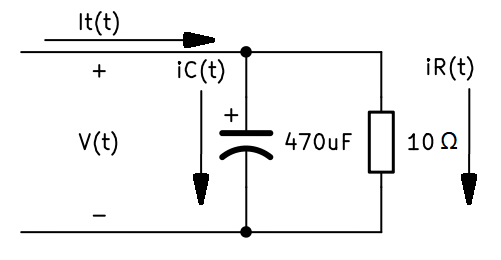
\includegraphics[scale=0.6]{./imagenes/CircuitoRC.png}
	\caption{Modelo de la salida de tensión.}
	\label{F:CircuitoRC}
\end{figure} \par 
Aplicando la ley de Kirchoff para los nodos:
\begin{equation}
i_t(t)=i_R(t)+i_C(t)
\end{equation}\par 
Pasando al dominio de Laplace:
\begin{equation}
I_t(s)=I_R(s)+I_C(s)
\end{equation}\par 
Reemplazando por lo obtenido anteriormente:
\begin{equation}
I_t(s)=\frac{V(s)}{R}+sCV(s)
\end{equation}\par 
Finalmente obtenemos el modelo que define la carga:
\begin{equation}
G_P(s)=\frac{V(s)}{I_t(s)}=\frac{1}{\frac{1}{R}+sC}
\end{equation}\par 
Con este y el lazo cerrado de corriente obtenido en la sección anterior es posible diseñar el control externo de tensión de forma tal que cumpla con ciertas especificaciones de diseño. Es posible utilizar la técnica de reubicación de polos por lugar geométrico de las raíces para obtener las constantes a implementar. \par 
La ecuación a diferencias a utilizar resulta en la presentada en \ref{eq:PIDp}.

\section{Algoritmo Anti-Windup}
La acción de control resultante del PI $u_{PI}(kT_s)$ puede ser saturada o limitada a valores positivos y/o negativos en casos en los que se presentan sobretensiones o sobrecorrientes por encima de los valores permitidos. La limitación de la acción de control a un valor fijo, significa que el sistema pierde la controlabilidad de los estados del proceso dado que sería similar a imponer un valor de referencia fijo; en este caso, esta referencia sería la del lazo interno de control de corriente. Esta situación provoca que el error entre la referencia y la salida varíe, tanto en sentido positivo como negativo, sin poder llevarlo a cero y por ende, al existir una acción de integración que acumula a cada periodo de muestreo, la misma puede crecer sin control, limitada únicamente por el tamaño de los registros que almacenen esta variable, con una excursión entre un valor máximo positivo a un valor máximo negativo, pasando el sistema lineal, a ser no lineal. Si esta situación no es controlada, puede provocar un comportamiento oscilatorio de los estados del proceso y si por acaso la acción de control vuelve a situarse dentro de los valores normales, puede que no vuelva a operar correctamente y deba reiniciarse el proceso. Este aumento sin control de la acción integral es lo que se denomina \textit{windup}, y es por lo que debe implementarse una acción \textit{anti-windup}. \par
Se opta por utilizar una forma simple de \textit{anti-windup} que consiste en que la integración del PI dada por $u_{PI}[(k-1)T_s]$ sea actualizada según el valor de saturación y los valores de los errores actual y anteriores, afectados por sus coeficientes. Esto provoca que a cada periodo de muestreo y mientras se mantenga limitada la acción de control, el error de tensión $e_v(kTs)$ se mantenga acotado y por ende también las variables de estados del proceso.
Matemáticamente, el algoritmo se representa de la siguiente manera:
\begin{itemize}
\item Condición 1: Valor mayor al valor de limitación positivo: \\
Si $u_{PI}(kT_s)\geq u_{PI\_ sat}$
\begin{equation}
	u_{PI}[(k-1)T_s]=u_{PI\_ sat}-K_{v1}\cdot e_v(kT_s)-K_{v2}\cdot [(k-1)T_s]-K_{v3}\cdot [(k-2)T_s]
\end{equation}

\item Condición 2: Valor menor al valor de limitación negativo. \\
Si $u_{PI}(kT_s)\leq -u_{PI\_ sat}$
\begin{equation}
	u_{PI}[(k-1)T_s]=-u_{PI\_ sat}-K_{v1}\cdot e_v(kT_s)-K_{v2}\cdot [(k-1)T_s]-K_{v3}\cdot [(k-2)T_s]
\end{equation}
\item Condición 3: Valor dentro de la región lineal \\
Si $u_{PI\_ sat}>u_{PI}(kT_s)>-u_{PI\_ sat}$
\begin{equation}
	u_{PI}[(k-1)T_s]=u_{PI}(kT_s)
\end{equation}
\end{itemize} \par 

Además, a cada periodo de muestreo, ya sea que la acción de control resulte limitada o no, debe actualizarse el error de tensión, o sea:
\begin{equation}
	e_v[(k-2)T_s]=e_v[(k-1)T_s] \qquad	e_v[(k-1)T_s]=e_v(kT_s)
\end{equation}
